\subsection{Opret sag}
	Dette afsnit vil indeholde en gennem gang af design, grafisk bruger interface og implentering af Opret sag activityen til android applikationen
	
	\subsubsection{Design}
	Opret sag er designet efter samme fremgangsmåde som opret bruger. Det kan ses på figur \vref{fig:OpretBrugerSekvens}. Hvor input felterne bliver valideret, og udfra dette gives der feedback til brugeren om eventuelle fejl. 
	Klasse relationerne er på samme måde som opret bruger og log ind bygget op omkring MVP, som kan ses på figur \vref{fig:Klasse diagram for Log Ind Android}.
	Dog med andre navne tilsvarende opret sag activity.
	
	\subsubsection{Grafisk Bruger Interface}
	Layouttet for Opret sag activityen som den ser ud på android applikationen.
	\begin{figure} [!ht]
		\begin{center}
			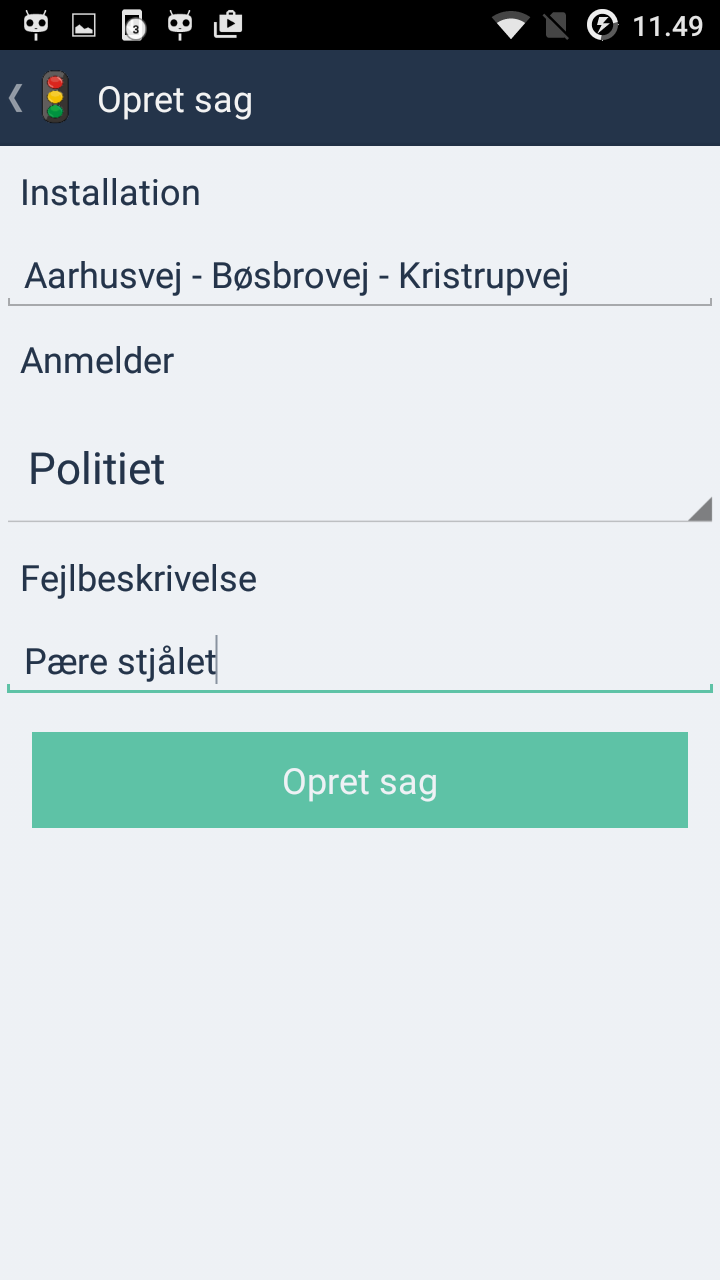
\includegraphics[height=10cm]{Android/Billeder/AndroidOpretSag}
		\end{center}
		\caption{Sekvens diagram for lyskryds oversigt på android appliktionen}
		\label{fig:Opret sag på android applikationen }
	\end{figure} \\
	Skal man have oprettet en sag, trykker man opret sags knappen på Home page, se figur \vref{fig: Traffic Control - Home Page}. Efter man har valgt opret sag på Home page, vises skærmenen som er vist ovenfor. \\
	
	\pagebreak
	
	\subsubsection{Implementering}
	Når en brugen forsøger at oprette en ny sag, validerer presenteren at der er indtastet information, inden at informationen bliver sendt videre til modellen. Hvis et felt ikke er udfyldt giver presenteren besked til viewet om at en fejlbesked om dette, skal vises. Hvis alle de påkrævet feltet er fyldt ud bliver et request sendt til API'et, gennem Modellen og DAL-laget.
	\\Der er implementeret autocomplete på feltet "Installation", som henter sine forslag for modellen. På samme måde hentes valgmuligheder til feltet "Anmelder" også fra modellen. \\